\documentclass[12pt,a4paper]{article}
\usepackage[UTF8]{ctex}     %先引入ctex
\usepackage[utf8]{inputenc} %再引入inputenc
\usepackage{graphicx}
\usepackage{geometry}
\usepackage{xcolor}
% \usepackage{lazylatex}
\usepackage{amsmath}
\usepackage{enumerate}
\usepackage{caption}
\usepackage{listings}
\captionsetup[lstlisting]{labelfont=bf,justification=justified}

\graphicspath{{img/}}
% 边距
\geometry{left=2.0cm,right=2.0cm,top=2.0cm,bottom=3.0cm}
% 大题
\newenvironment{problems}{\begin{list}{}{\renewcommand{\makelabel}[1]{\textbf{##1}\hfil}}}{\end{list}}
% 小题
\newenvironment{steps}{\begin{list}{}{\renewcommand{\makelabel}[1]{##1.\hfil}}}{\end{list}}
% 答
\providecommand{\ans}{\textbf{答}:~}
% 解
\providecommand{\sol}{\textbf{解}.~}

\usepackage[colorlinks,linkcolor=blue]{hyperref}
\usepackage{bookmark}
\providecommand{\code}[2]{\lstinputlisting[language=#2,caption=\href{run:#1}{\ttfamily #1}]{#1}}

% listings
\definecolor{grey}{rgb}{0.8,0.8,0.8}
\definecolor{darkgreen}{rgb}{0,0.3,0}
\definecolor{darkblue}{rgb}{0,0,0.3}
\lstset{%
    % numbers=left, %行号
    % numberstyle=\tiny\color{grey},
    showstringspaces=false,
    showspaces=false,%
    tabsize=4,%
    frame=shadowbox,%
    basicstyle={\ttfamily\scriptsize},%
    keywordstyle=\color{blue!80!black}\bfseries,%
    identifierstyle=,%
    commentstyle=\color{green!50!blue}\itshape,%
    stringstyle=\color{green!50!black},%
    rulesepcolor=\color{gray!20!white},
    breaklines,
    columns=flexible,
    extendedchars=false,
    %mathescape=true,
}

\begin{document}
\title{\normalsize \underline{操作系统(D)}\\\LARGE 项目 1}
\author{Log Creative }
\date{\today}
\maketitle

\begin{problems}
    \item[一] \textbf{创建内核模块}
    \begin{steps}
        \item[1] 列出当前加载的所有内核模块。
        
        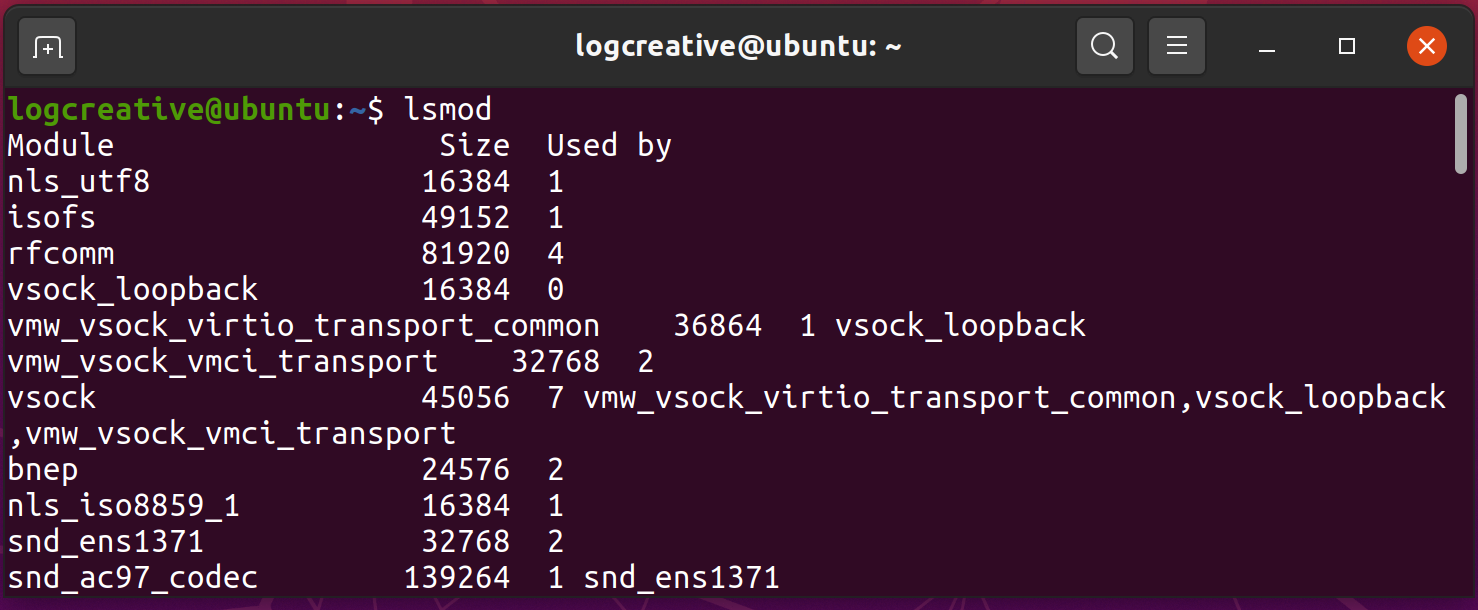
\includegraphics[width=0.88\textwidth]{lsmod.png}

        \item[2] 编写模块以输出提示:

        \begin{lstlisting}[language=c]
int simple_init(void){
    printk(KERN_INFO "Loading Module\n");
    return 0;
}

void simple_exit(void){
    printk(KERN_INFO "Removing Module\n");
}
        \end{lstlisting}

        使用 MakeFile 编译:
        \code{src/Makefile}{}

        \item[3] 加载与卸载内核模块
        
        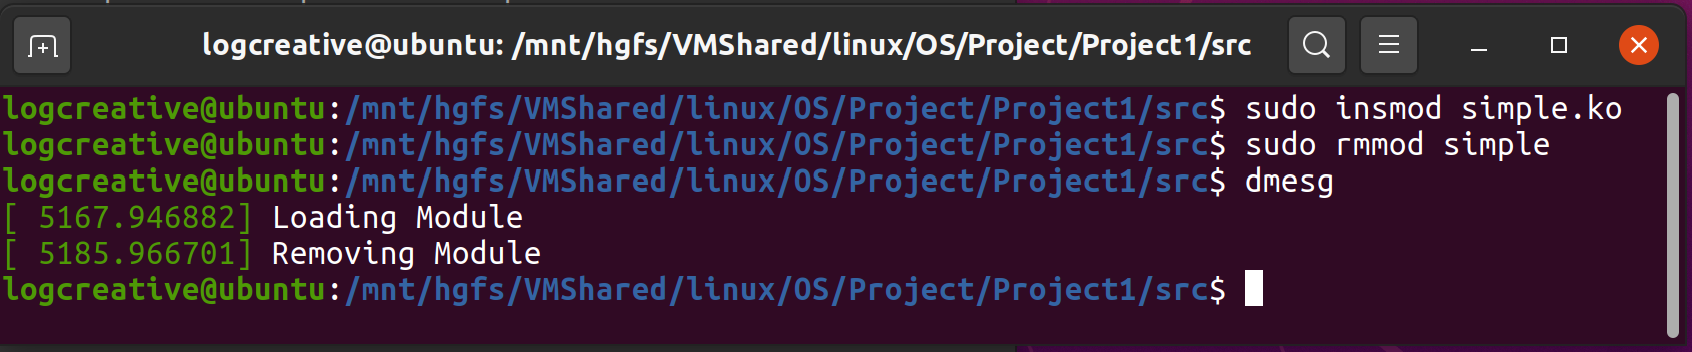
\includegraphics[width=0.88\textwidth]{insmod.png}

        添加了两行代码用于打印 \texttt{GOLDEN\_RATIO\_PRIME} 和 3300 与 24 的最大公因数:

        \begin{lstlisting}[language=c]
// @ simple_init(void)
printk(KERN_INFO "%lu\n", GOLDEN_RATIO_PRIME);

// @ simple_exit(void)
printk(KERN_INFO "%lu\n", gcd(3300,24));
        \end{lstlisting}

        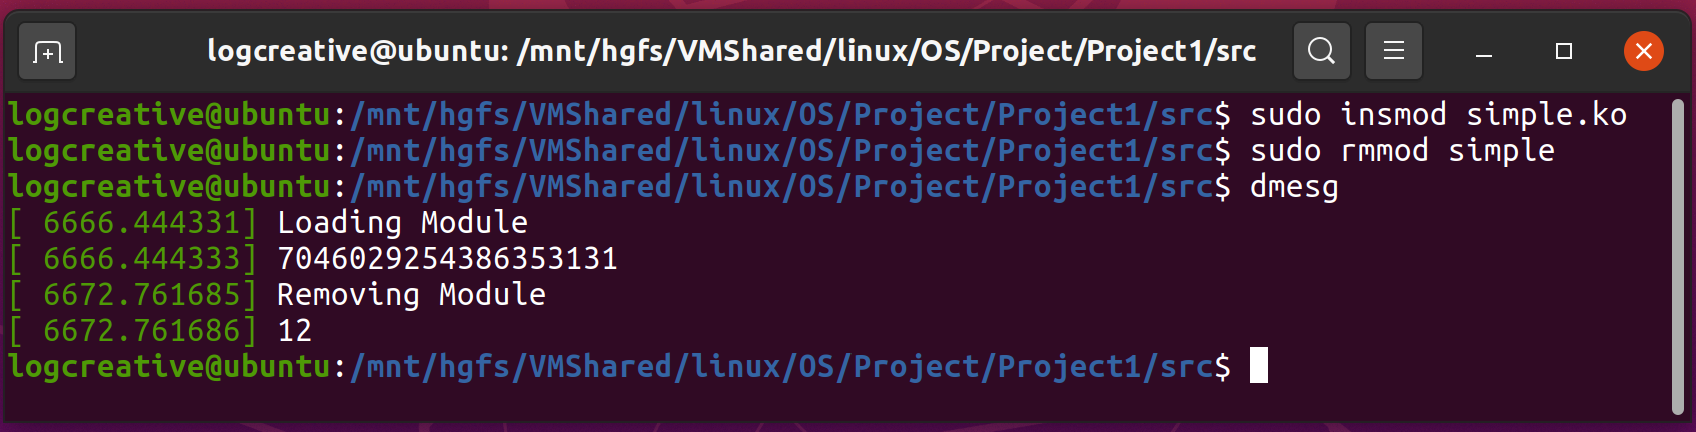
\includegraphics[width=0.88\textwidth]{msimple.png}

        继续添加代码用于打印 \texttt{jiffies} 和 \texttt{HZ}。
        \begin{lstlisting}[language=c]
// @ simple_init(void)
printk(KERN_INFO "%lu\n", jiffies);
printk(KERN_INFO "%u\n", HZ);

// @ simple_exit(void)
printk(KERN_INFO "%lu\n", jiffies);
        \end{lstlisting}

        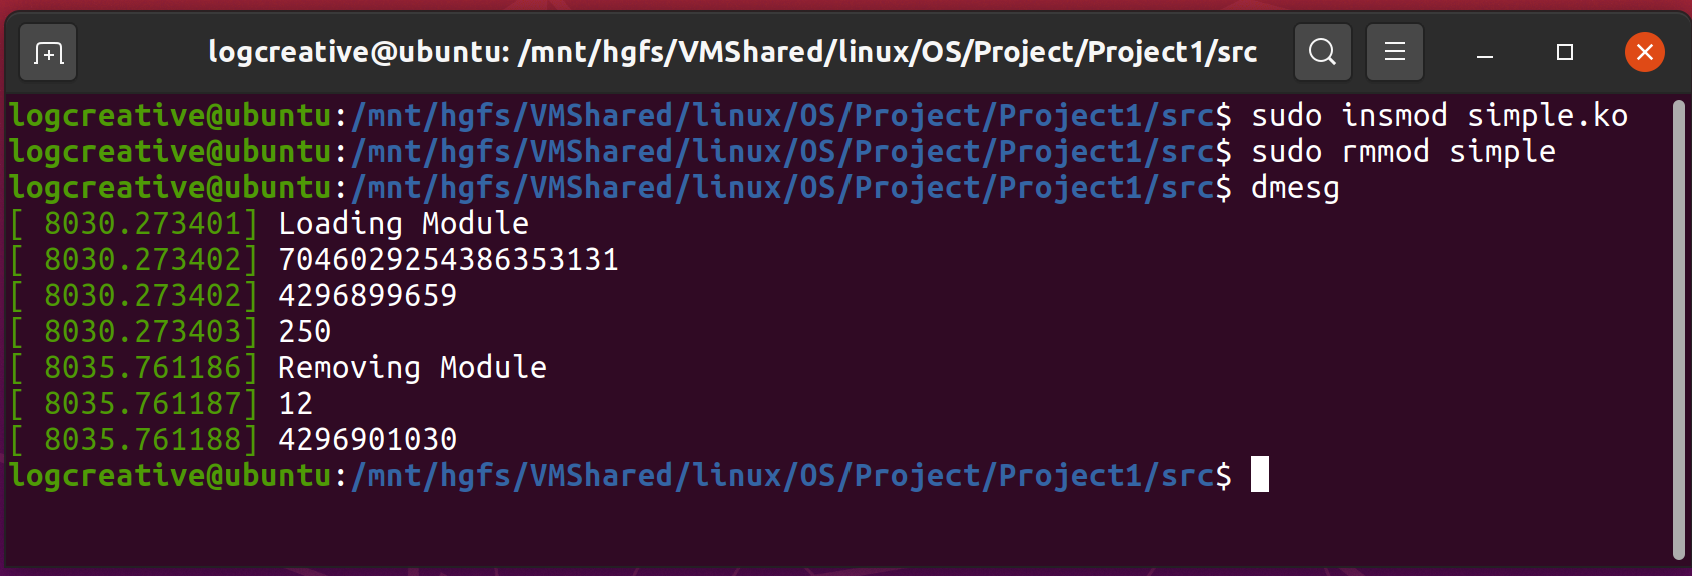
\includegraphics[width=0.88\textwidth]{jiffies.png}

        最后该部分所有的代码如下:
        \code{src/simple.c}{c}

    \end{steps} 
    \item[二] \verb"\proc" \textbf{文件系统}
    
    使用 \verb"\proc" 文件系统打印 Hello World。

    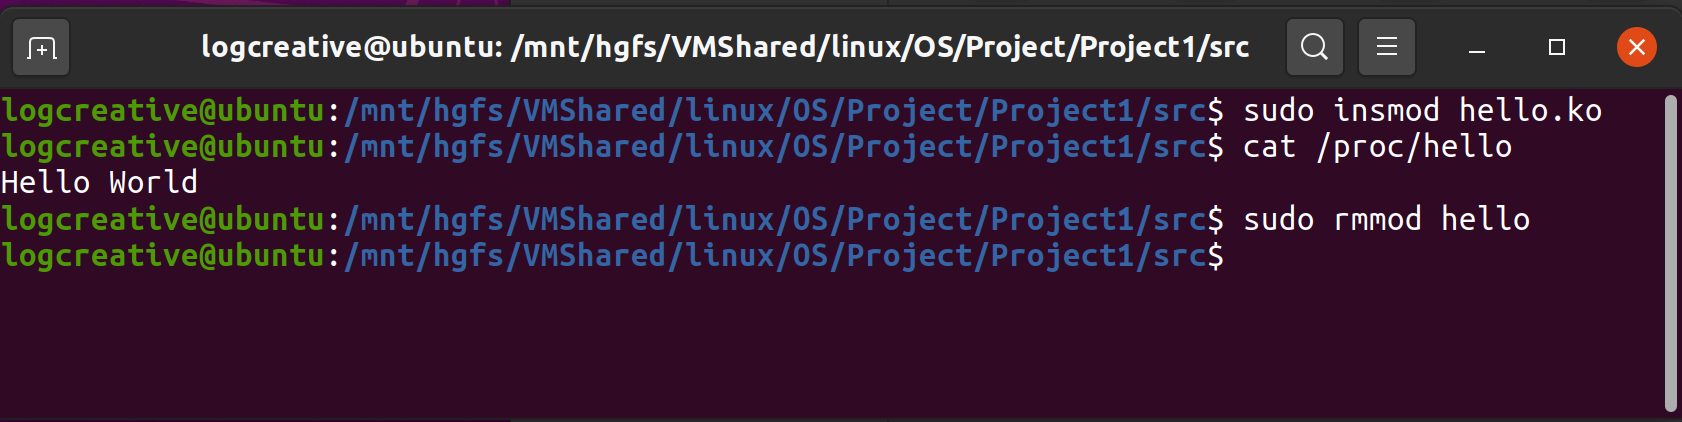
\includegraphics[width=0.88\textwidth]{hello.png}

    由于采用了 Ubuntu 20.04 系统,所以使用的是 Linux 内核,因此需要使用 \texttt{proc\_ops} 结构体来传入 \texttt{proc\_create} 的第四参数。

    \code{src/hello.c}{c}

    \item[三] 作业
    \begin{steps}
        \item[1] 使用 \verb"\proc" 打印 \texttt{jiffies}。
        
        最重要的部分是更改了 \verb"sprintf" 的所在行。
        \begin{lstlisting}
            rv = sprintf(buffer,"%lu\n",jiffies);    
        \end{lstlisting}

        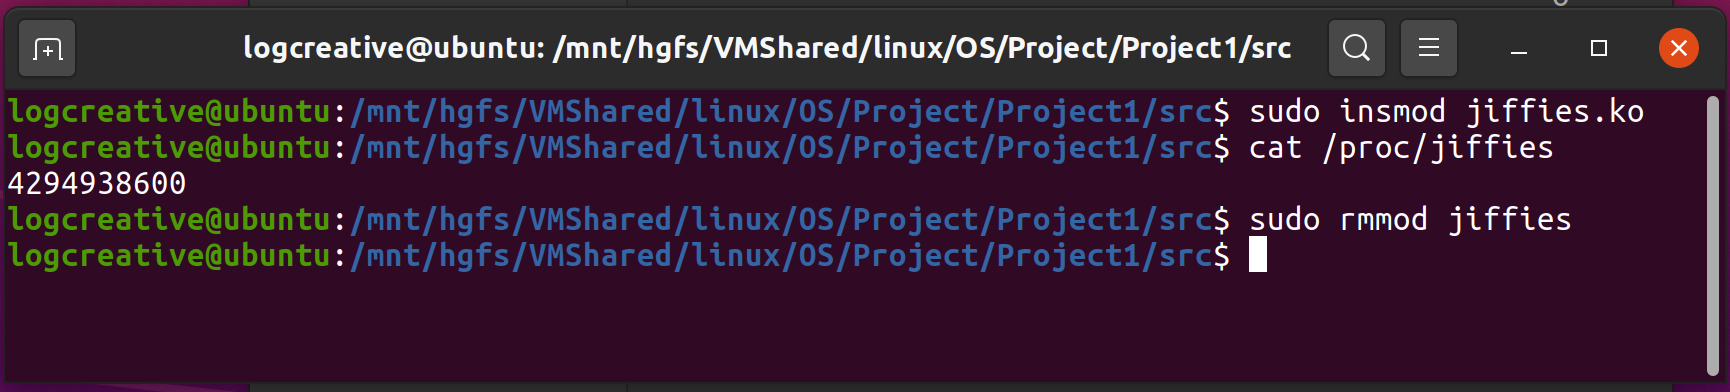
\includegraphics[width=0.88\textwidth]{jiffiesh.png}
        
        \code{src/jiffies.c}{c}

        \item[2] 使用 \verb"\proc" 打印模块运行秒数。
        
        初始时初始化 \verb"init_jiff" 变量,秒数由 \verb"HZ" 计算得到:
        \begin{equation*}
            \texttt{seconds} = \frac{\texttt{jiffies}-\texttt{init\_jiff}}{\texttt{HZ}}
        \end{equation*}
        
        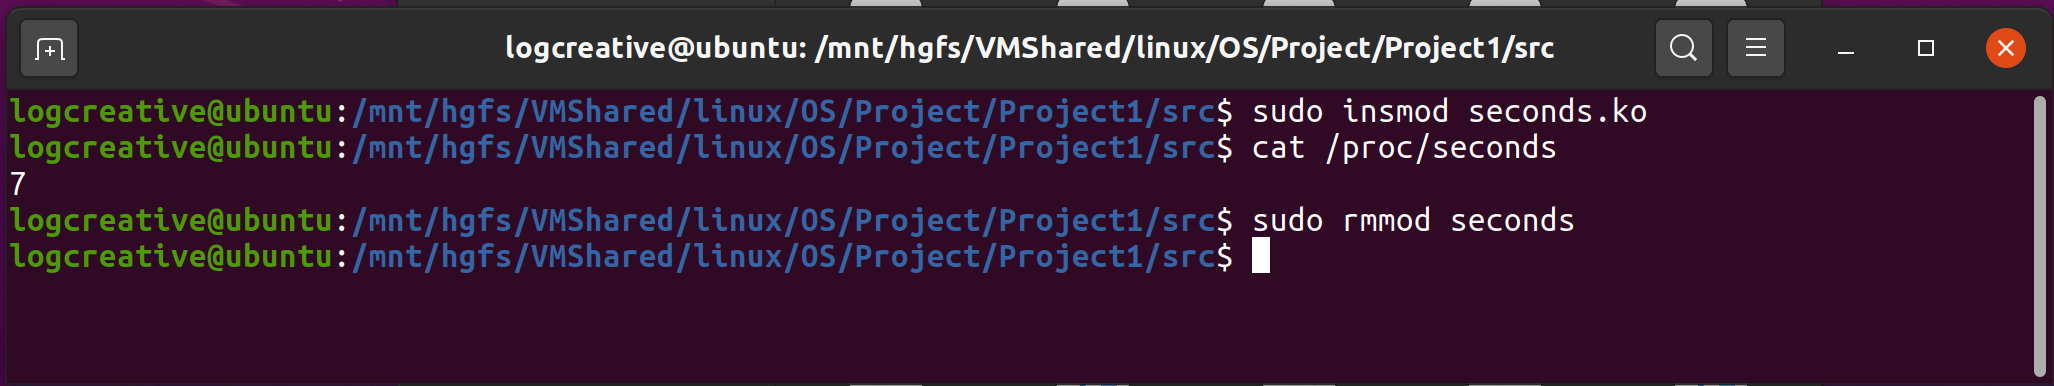
\includegraphics[width=0.88\textwidth]{seconds.png}

        \code{src/seconds.c}{c}
    \end{steps}

\end{problems}


\end{document}
